
\begin{titlepage}
\begin{center}

% Upper part of the page. The '~' is needed because \\
% only works if a paragraph has started.
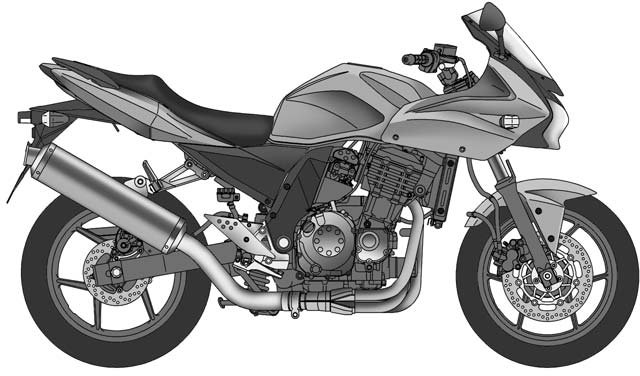
\includegraphics[scale=0.5]{global/project_logo.jpg}

\textsc{\LARGE Jonathan S. Romero}\\[1.5cm]

\textsc{\Large presents }\\[0.5cm]

% Title
\HRule \\[0.4cm]
{ \huge \bfseries Arduino based Motorcycle Gauge Cluster}\\[0.4cm]

\textsc{\Large  for 2005 Kawasaki Z750s}\\[0.5cm]

\HRule \\[1.5cm]

% Author and supervisor
\begin{minipage}{0.4\textwidth}
\begin{flushleft} \large
\emph{Author:}\\
Jonathan \textsc{Romero}
\end{flushleft}
\end{minipage}

\vfill

% Bottom of the page
{\large \today}

\end{center}
\end{titlepage}
